%----------------------------------------------------------------------------
\label{side}
%----------------------------------------------------------------------------
Consider an optical setup where a laser beam line is intersected orthogonally at its focus by a receiver beam line. Let a coordinate system be centered at the intersection where the z-axis corresponds to the receiver beam line and the x-axis corresponds to the laser beam line (see Figure \ref{side_view_figure}). Ray bundles (corresponding to the sensitive phase space region for the CT103 monochromator) are transformed to the intersection and the overlap with focused laser beam is determined. Based on that overlap, an ``excited sensitive volume'' is defined at the target region for various two--lens combinations in the receiver beam line. The overlap will naturally include any cropping of phase space in the angular dimension. A solid angle of acceptance is defined and the excited sensitive volume is scaled by the ratio of this solid angle over $4\pi$. The surface formed by this scaled volume (as a function of lens focal lengths) is used to determine the optimal lens combination for laboratory scale versions of the side view geometry. See Figure \ref{side_view} for a resulting surface applicable to a bench top experiment.
%----------------------------------------------------------------------------
%----------------------------------------------------------------------------
%bb defines the bounding box for the pdf
%viewport defines the area of the pdf used
%in sidewaysfigure the last entry in bb moves the caption toward/away the pic
%in sidewaysfigure the second entry in bb moves the pic toward/away the caption
%----------------------------------------------------------------------------
\begin{figure}
\scalebox{0.7}[0.7]{
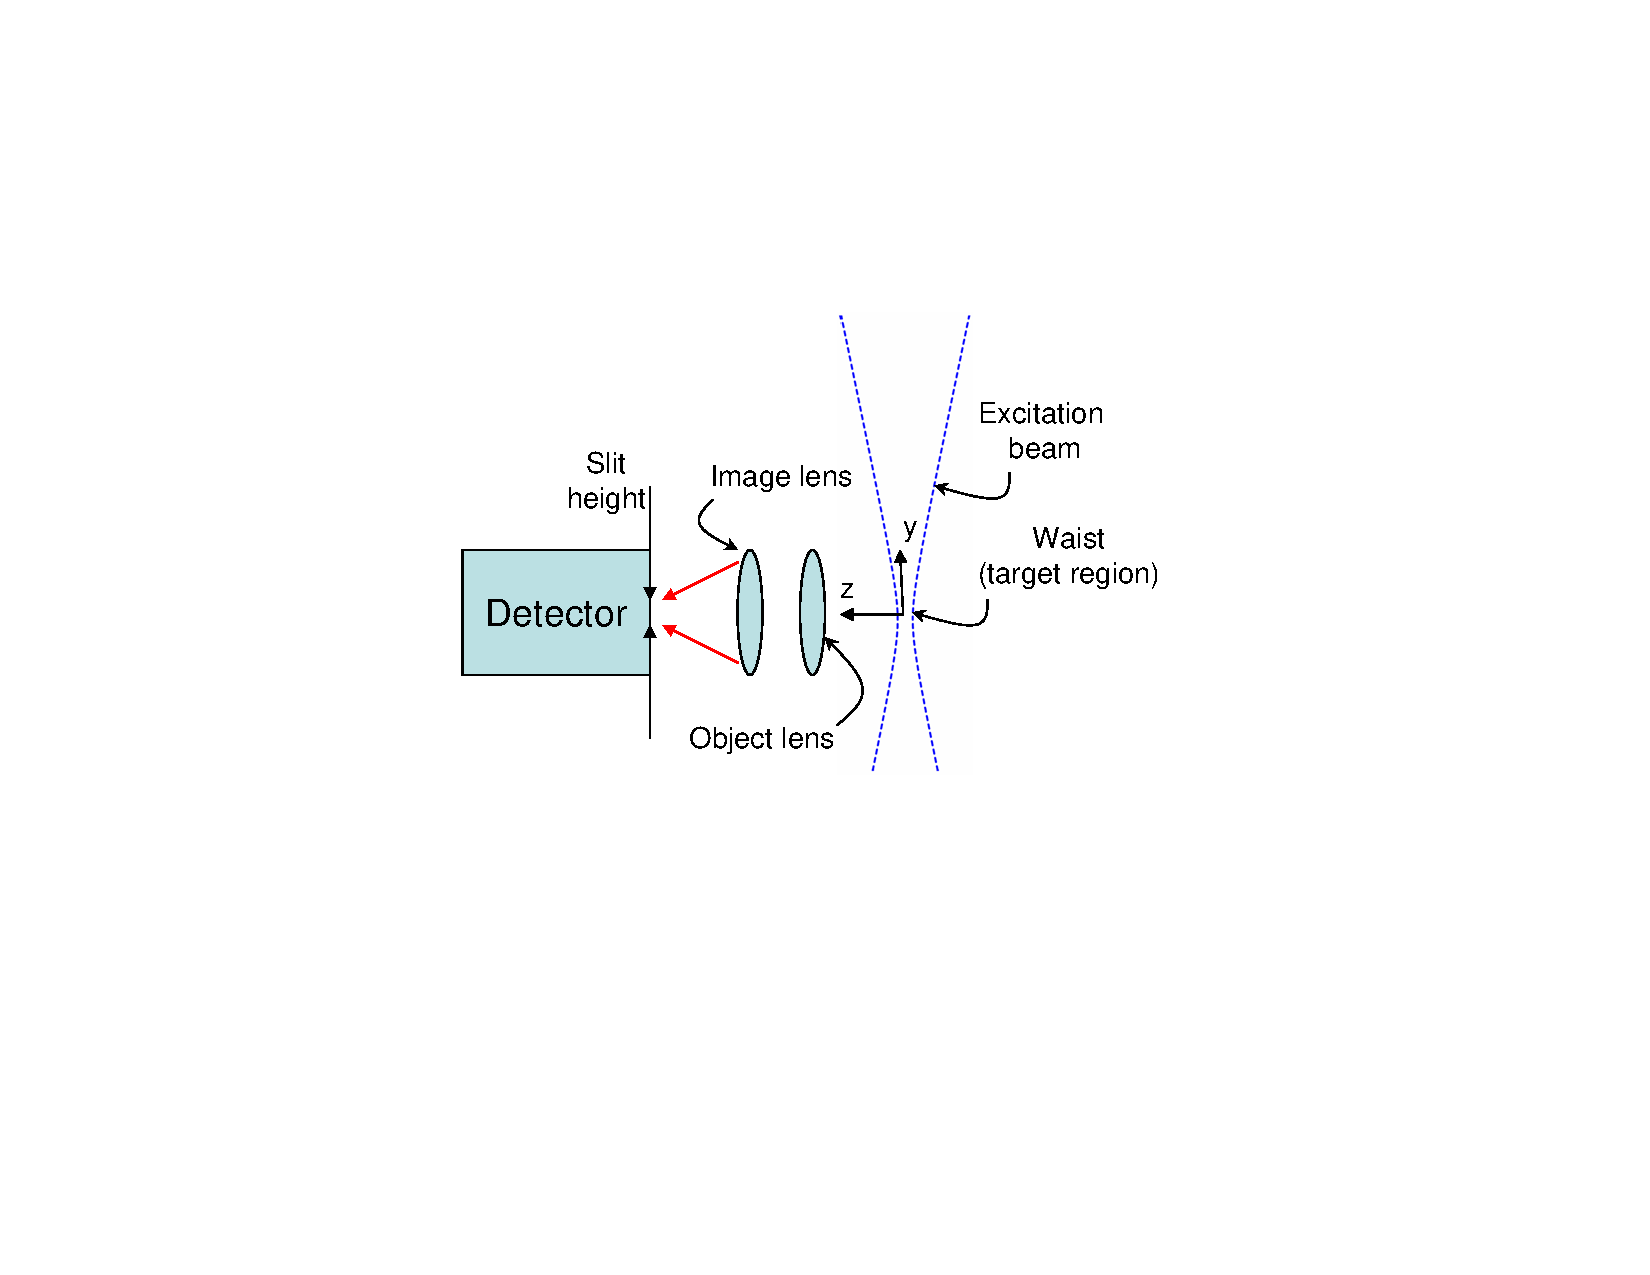
\includegraphics[bb=80 230 489 450]
{side_view_figure/side_view_figure.pdf}
}
\caption[Side view geometry]{Side view geometry. For the calculation in Figure \ref{side_view}, each object (image) lens is placed one focal length from the target region (detector input). The slit such that its long dimension (height) is oriented in the y--direction and its narrow dimension is oriented in the x--direction.}
\label{side_view_figure}
\end{figure}
%----------------------------------------------------------------------------

%----------------------------------------------------------------------------
%----------------------------------------------------------------------------
%----------------------------------------------------------------------------
%bb defines the bounding box for the pdf
%viewport defines the area of the pdf used
%in sidewaysfigure the last entry in bb moves the caption toward/away the pic
%in sidewaysfigure the second entry in bb moves the pic toward/away the caption
%----------------------------------------------------------------------------
\begin{figure}
\scalebox{0.7}[0.7]{
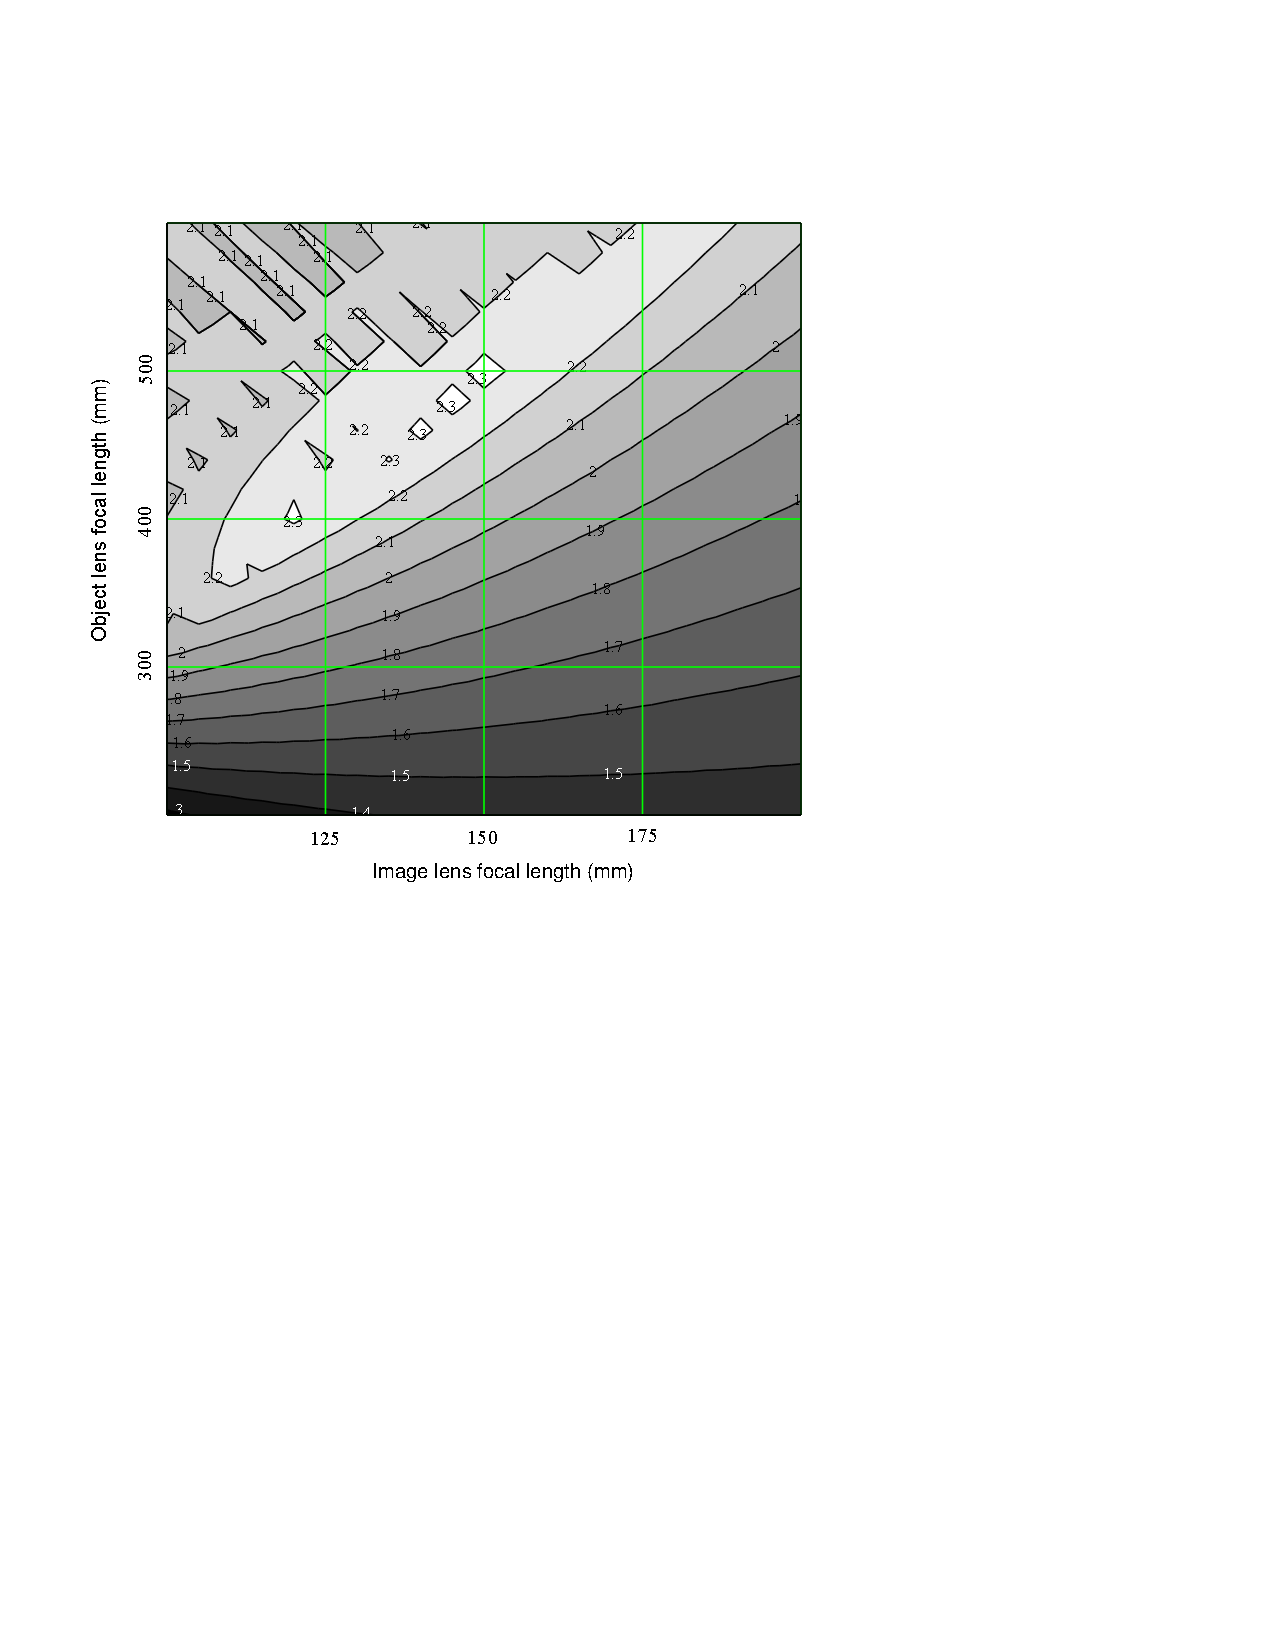
\includegraphics[bb=-60 360 489 725]
{side_view/side_view.pdf}
}
\caption[Side--view lens optimization surface]{Side--view lens optimization surface. For this calculation the beam waist diameter is 1 mm, the wavelength is 0.63 $\mu$m, the slitwidth is 300 $\mu$m, the slit height is 0.5 cm, and the monochromator acceptance angle is 52 mrad. The object lens is placed one focal length from the sample, while the image lens is placed one focal length from the monochromator input. The units for the contour in the plot are $10^{-12}$ m$^3$ (scaled volume). Thus if the target was air (near $10^{25}$ molecules per cubic meter) we would expect this system to be sensitive to $10^{13}$ atmospheric molecules (assuming all molecules decay optically in an isotropic fashion).}
\label{side_view}
\end{figure}
%----------------------------------------------------------------------------

%----------------------------------------------------------------------------

Suppose we choose a symmetric pair of 200mm lenses (i.e. unity magnification), now we can examine the dynamic and geometric effects of the velocity distribution on the detection system. Using the same geometry as above, we construct a rectangular region at the intersection to represent the sensitive volume with respect to the detection system (the ``sensitive'' volume). The height of the region in the y--direction is equal to the height of the monochromator input slit. The width of the region in the z--direction and x--direction is equal to the width of the monochromator input slit. Laser beam excitation of the region is modeled by a second rectangular region (also centered at the intersection) which is temporally switched (top hat envelope with a width equal to the laser pulse length). The width of the region in the z--direction and x--direction is equal to the waist diameter of the laser beam. The height of the region in the y--direction is equal to the Rayleigh range of the laser beam.

%----------------------------------------------------------------------------
%----------------------------------------------------------------------------
%bb defines the bounding box for the pdf
%viewport defines the area of the pdf used
%in sidewaysfigure the last entry in bb moves the caption toward/away the pic
%in sidewaysfigure the second entry in bb moves the pic toward/away the caption
%----------------------------------------------------------------------------
\begin{figure}
\scalebox{0.8}[0.8]{
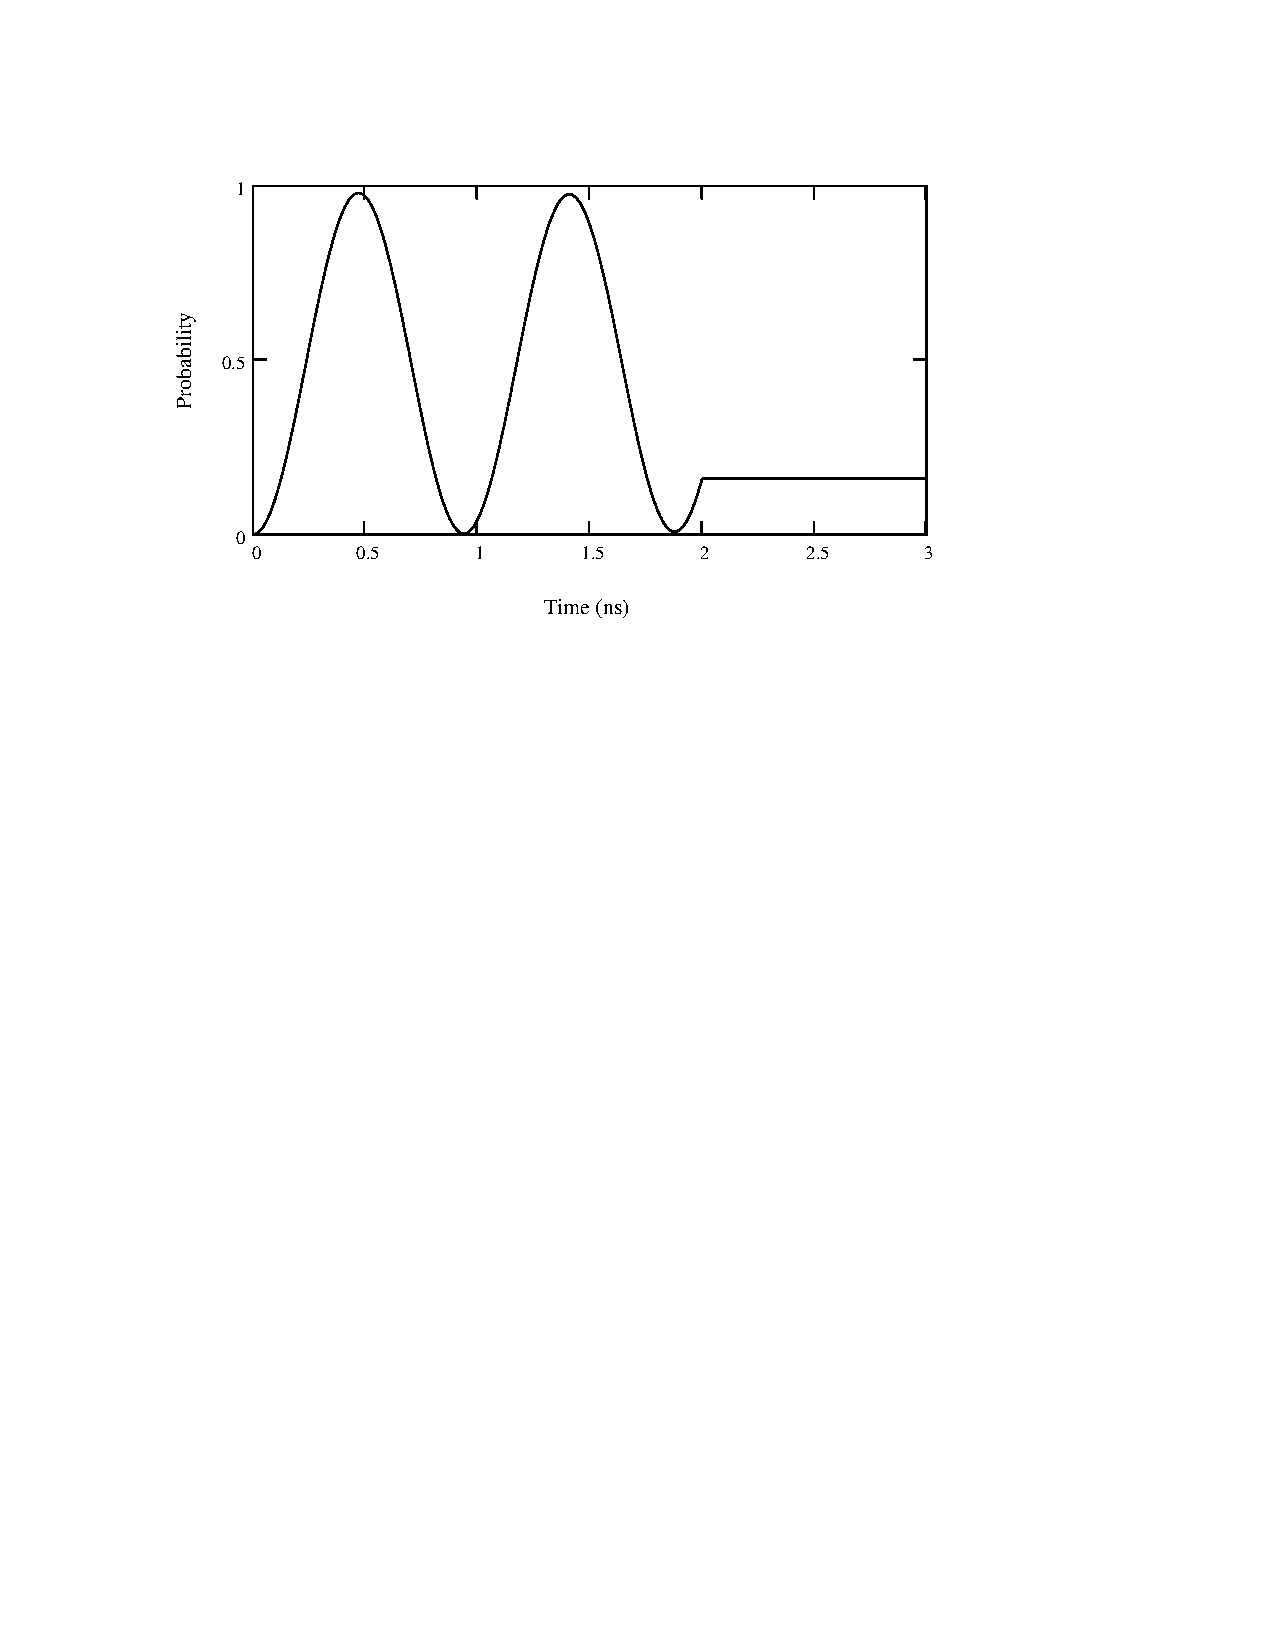
\includegraphics[bb=10 490 550 690]
{thermal_2/thermal_2.pdf}
}
\caption[Simulated thermal (Doppler and geometric) effects on observed fluorescence -- 2 ns pulse]{Simulated thermal (Doppler and geometric) effects on observed fluorescence -- 2 ns pulse. For this simulation a top hat pulse (temporal and spatial) with duration 2 ns, fluence of 1000 J/m$^2$, and beam diameter 1 mm (about 1 mJ per pulse), excites a thermal molecular iodine gas, with dipole matrix element $3.6\cross10^{-32}$ Cm (including FCF), at T = 293K.  The axial dimension of the sensitive region is set to 300 $\mu$m; this is set to the slit width, which is selected such that the J-splitting in iodine fluorescence can still be resolved. The transverse dimension of the sensitive region is set to 0.5 cm (slit mask).}
\label{thermal_2}
\end{figure}
%----------------------------------------------------------------------------

%----------------------------------------------------------------------------
%----------------------------------------------------------------------------
%----------------------------------------------------------------------------
%bb defines the bounding box for the pdf
%viewport defines the area of the pdf used
%in sidewaysfigure the last entry in bb moves the caption toward/away the pic
%in sidewaysfigure the second entry in bb moves the pic toward/away the caption
%----------------------------------------------------------------------------
\begin{figure}
\scalebox{0.8}[0.8]{
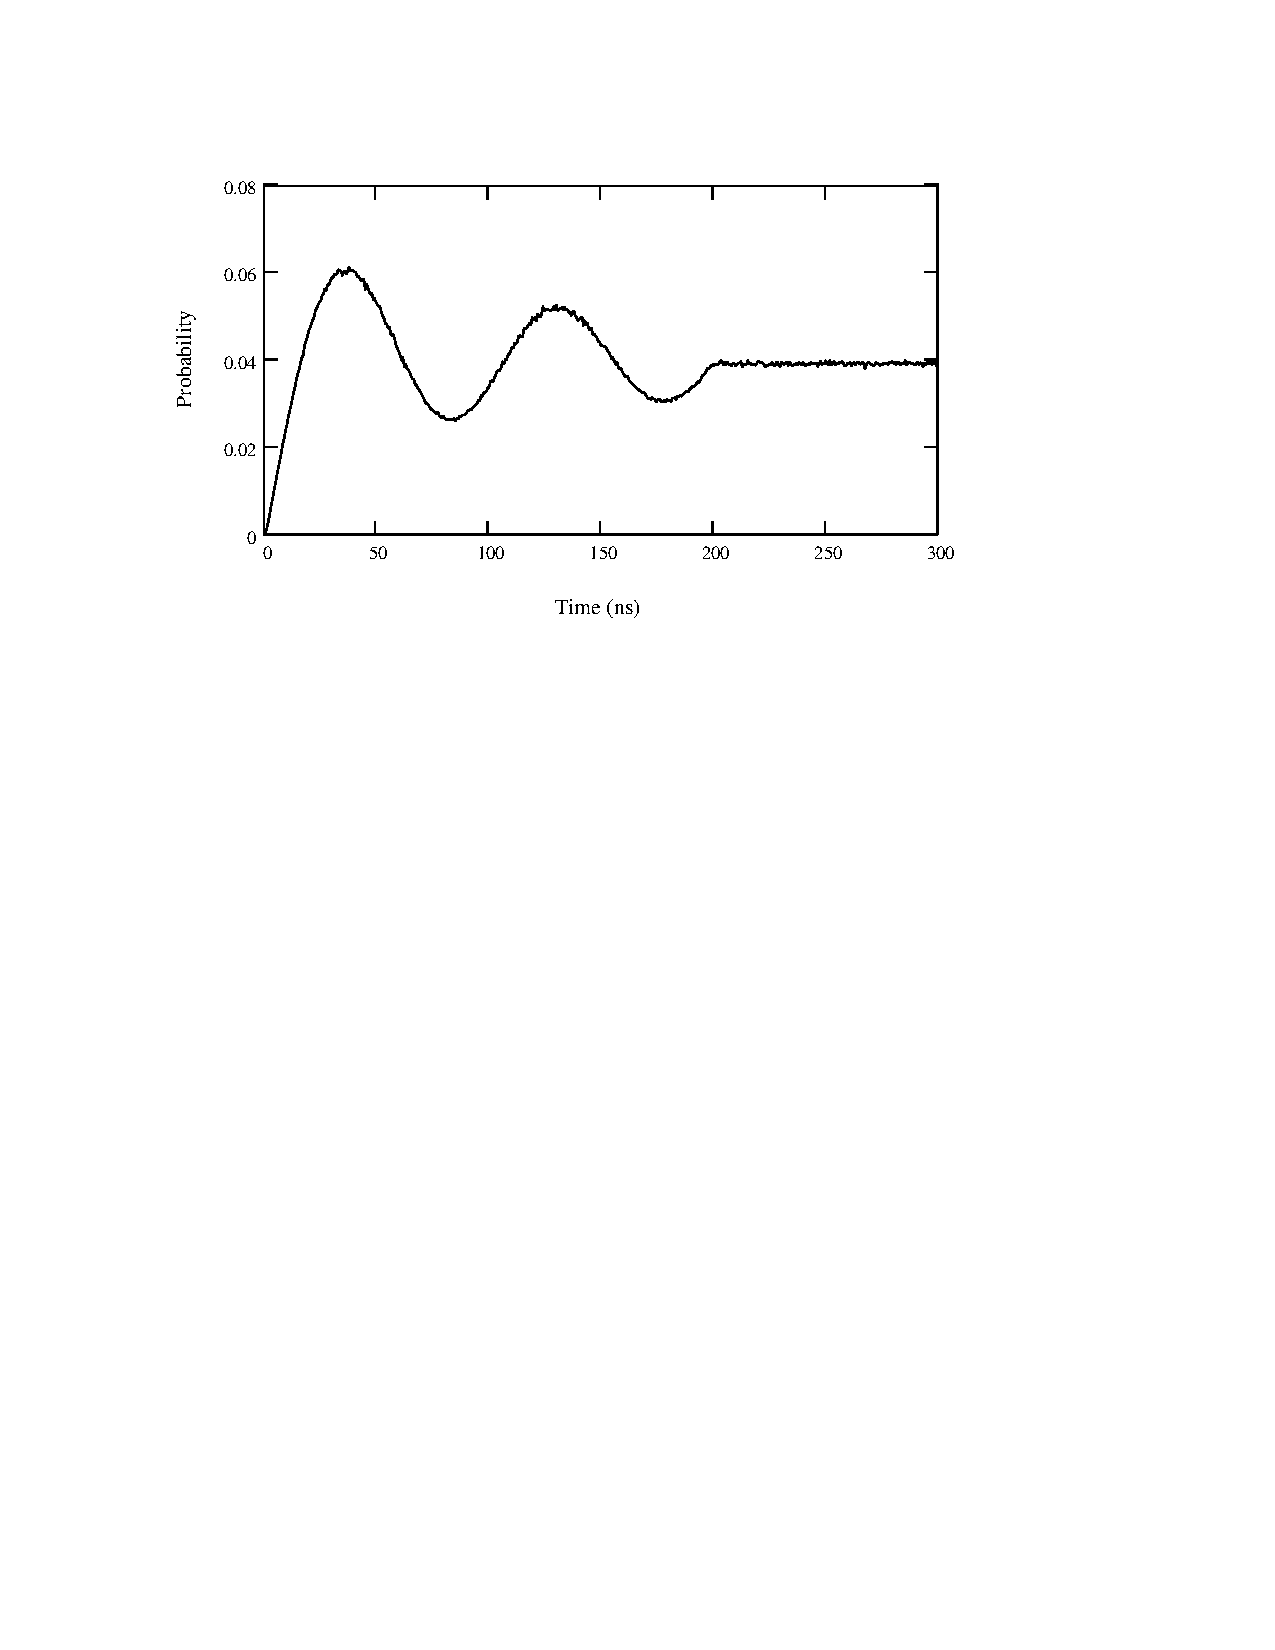
\includegraphics[bb=10 490 550 690]
{thermal_200/thermal_200.pdf}
}
\caption[Simulated thermal (Doppler and geometric) effects on observed fluorescence -- 200 ns pulse]{Simulated thermal (Doppler and geometric) effects on observed fluorescence -- 200 ns pulse. The calculations presented here have nearly the same parameters as Figure \ref{thermal_2} (left is ideal, right is polarization averaged) except these require a smaller fluence of 10 J/m$^2$ to induce two complete oscillations in 200 ns (instead of 1000 J/m$^2$ for 2 ns). The peak power of the pulse is 50 W -- four orders of magnitude larger than the typical CW HeNe laser.}
\label{thermal_200}
\end{figure}
%----------------------------------------------------------------------------

%----------------------------------------------------------------------------
An ensemble of molecules is generated in the sensitive region and tracked backwards in time, starting from some time $t$, to determine the average effect of molecular velocity on the ensemble dynamics at some instant. The ensemble is uniformly distributed in the volume and given the Maxwell-Boltzmann speed distribution (the velocities are isotropic). Each member of the ensemble is ballistically tracked and the duration and delay of its exposure to the excitation volume is recorded. The evolution of the (two level) molecule is calculated according to Equation \ref{final eom} and; thus, by averaging over the entire ensemble, the average probability of inversion is calculated for molecules in the detector's sensitive region at time $t$. This is repeated for many times $t$ to track the average behavior of the ensemble for some time interval. See Figures \ref{thermal_2} and \ref{thermal_200} for some results applicable to a bench top experiment. Comparing these two Figures to Figure \ref{doppler_only} we see that geometric effects are insignificant when using relatively large waists (and the molecules are relatively heavy and slow like iodine).

Even if we assume all of the inverted molecules decay optically, the collisional decay rate places limits on the number of photons emitted from the ensemble. If the collision rate dominates, it can be shown that (personal communication, Pui K. Lam, June 2006)
%----------------------------------------------------------------------------
\begin{equation}
n
=
\frac
{\tau_c}
{\tau_s}
N
\end{equation}
%----------------------------------------------------------------------------
where $n$ is the number of emitted photons, $\tau_c$ is the collision life time, $\tau_s$ is the spontaneous life time, and $N$ is the number of inverted molecules. Using the above results we can obtain an estimate for the number of photons captured in the detection system. Assuming the density of molecular iodine at 293K is near $10^{21}$ per m$^3$, the scaled volume (from Figure \ref{side_view}) is near $2\cross10^{-12}$ m$^3$, the maximum inversion probability is near $6\cross 10^{-2}$ (down from around 0.6 -- see Figure \ref{thermal_200}), and $\tau_c/\tau_s=0.1\cross10^{-6}/7\cross10^{-3}\sim1\cross10^{-5}$ ($\tau_s$ is derived using the same matrix element mentioned in the caption of Figure \ref{thermal_2}); then the total number of photons captured in the monochromator should be near 1200. It should be noted that for the 2 ns pulse (Figure \ref{thermal_2}), even though the maximum inversion probability (0.6) is an order of magnitude larger; the ratio $\tau_c/\tau_s=1\cross10^{-9}/7\cross10^{-3}\sim1\cross10^{-7}$ is two orders of magnitude \emph{smaller} for a reduced number of captured photons when compared to the 200 ns pulse.
%----------------------------------------------------------------------------
